%\section{Versuchsaufbau}
%\label{sec:Versuchsaufbau}
%
%
\section{Durchführung}
\label{Durchführung}
Zur Durchführung des Versuchs liegt ein LRC-Messgerät, ein Signalgenerator, ein NIM-Pulser und ein Oszilloskop vor.
Außerdem sind mehrere Koaxialkabel zur Untersuchung vorhanden sowie ein Kasten mit verschiedenen Abschlüssen. 
Die Kabel haben jeweils eine Dielektrizität von~\cite{V52}
\begin{equation}
    \epsilon_{r} = 2,25 \, .
    \label{eqn:dieltheo}
\end{equation}
Es werden sechs verschiedene Kabel untersucht, deren Längen in \autoref{tab:lentheo} zu finden sind.
Bei Kabel 5 handelt es sich um ein $\qty{75}{\ohm}$ Kabel, die restlichen Kabel sind $\qty{50}{\ohm}$ Kabel.
\begin{table}[H]
    \centering
    \caption{Genaue Längen der verwendeten Koaxialkabel.}
    \begin{tabular}{cc}
    \toprule
    Kabel& $l \,/\, [\unit{\meter}]$ \\
    \midrule
    1  & 84 \\
    2  & 5\\
    3  & 10\\
    4  & 1,5\\
    5  & 10\\
    6  & 1,15\\
    \bottomrule
    \end{tabular}
    \label{tab:lentheo}
\end{table}
\FloatBarrier\noindent
Zunächst wird bei Kabel 3 die Frequenzabhängigkeit der Leitungskonstanten $L$, $R$ und $C$ gemessen und daraus der Betrag der Impedanz $\left|Z\right|$ sowie der Phasenversatz $\varphi$ bestimmt. 
Dazu wird das Kabel direkt an das LRC-Messgerät angeschlossen.
Die Messung wird für Frequenzen von $\qty{1}{\kilo\hertz}$ bis $\qty{100}{\kilo\hertz}$ durchgeführt.
Das Gerät kann keine Frequenzen zwischen $\qty{20}{\kilo\hertz}$ und $\qty{100}{\kilo\hertz}$ vermessen, weshalb ein Sprung in der Messreihe gemacht werden muss. 
Für die Messung von $L$ und $R$ muss an das Ende des Kabels ein Kurzschluss angeschlossen werden. Für die Messung von $C$ bleibt das Ende offen. 
\\\\
Nun wird für die Messung der Kabellängen, Dämpfungskonstanten und Dielektrizitäten der Aufbau in \autoref{fig:aufbau} aufgebaut.
Dabei wird der NIM-Pulser verwendet und die sechs verschiedenen Kabel nacheinander mittels T-Stück und weiterem kurzen Kabel an Oszilloskop und Pulser angeschlossen.
Für jedes Kabel wird der zeitliche Abstand $\increment t$ zwischen ausgehendem und reflektiertem Puls sowie die Amplituden der beiden Pulse gemessen.
Dazu wird der Curser am Oszilloskop verwendet. 
Aus den Werten können dann die drei Größen bestimmt werden.
\\\\
Als nächstes sollen verschiedene Abschlüsse untersucht werden. 
Dazu wird ebenfalls der Aufbau in \autoref{fig:aufbau} mit dem Kabel 3 verwendet. 
Als Pulser wird der Signalgenerator genutzt.
An diesem wird eine Recheckspannung eingestellt.
Es werden dann nacheinander die Abschlüsse 1, 2, 3, und 8 des Kastens sowie ein offener Abschluss, ein Kurzschluss, ein $\qty{50}{\ohm}$ und ein $\qty{75}{\ohm}$ Widerstand als Abschluss angeschlossen.
Für jeden Abschluss wird das Signalbild am Oszilloskop abgespeichert. 
Dieses kann dann mit den theoretischen Verläufen abgeglichen werden und es kann die Signalspannung abgelesen werden.
\\\\
Zur Messung der Reflexionsfaktoren bei Reihenschaltung eines $\qty{50}{\ohm}$ und eines $\qty{75}{\ohm}$ Kabels wird ebenfalls der Aufbau in \autoref{fig:aufbau} benutzt. 
Hier wird Kabel 3 direkt am Oszilloskop angeschlossen und das Ende von Kabel 3 mit Kabel 5 durch entsprechenden Adapter verbunden. 
Das andere Ende von Kabel 5 bleibt offen.
Als Pulser wird wieder der Signalgenerator verwendet, wobei Pusle als Signalspannung gewählt werden.
Am Oszilloskop kann dann die Amplitue des Ausgangspulses und der reflektierten Pulse gemessen werden.
Daraus lassen sich die Reflexionsfaktoren bestimmen.
\begin{figure}
    \centering
    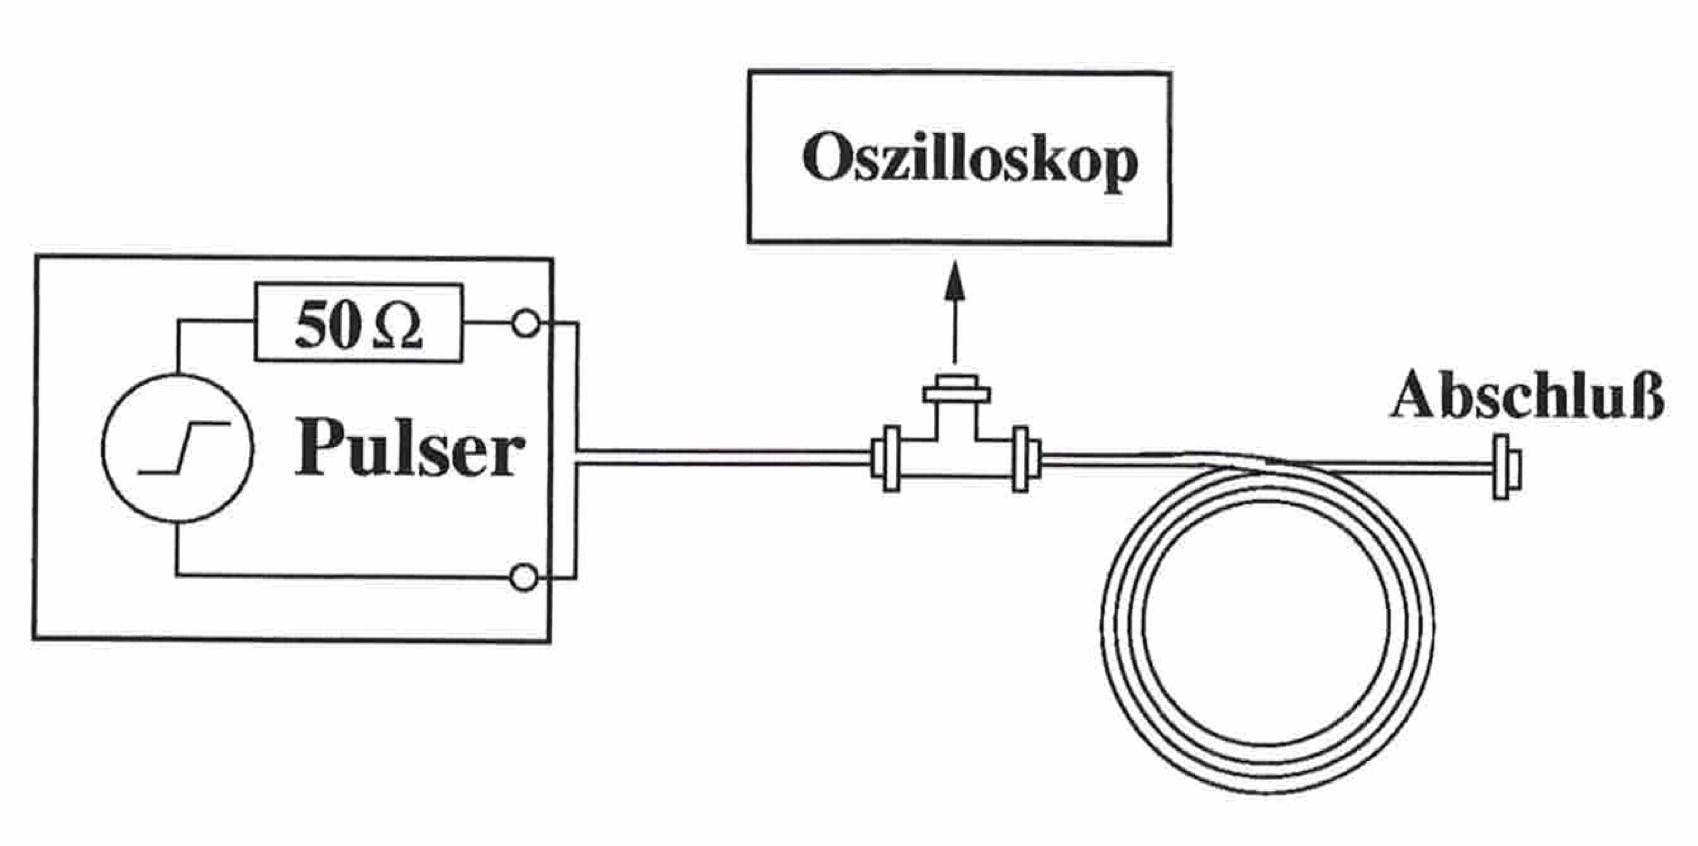
\includegraphics[width=0.5\textwidth]{content/images/aufbau.jpeg}
    \caption{Versuchsaufbau für die Messung der Kabellängen, Dämpfungskonstanten, Dielektrizitäten, Abschlüsse und Reflexionsfaktoren \cite{V52}.}
    \label{fig:aufbau}
\end{figure}